% Schaltungstechnik Formelsammlung für ST2 SoSe 2011
% 2 Seiten

% Dokumenteinstellungen
% ======================================================================

% Dokumentklasse (Schriftgröße 6, DIN A4, Artikel)
\documentclass[6pt,a4paper]{scrartcl}

% Pakete laden
\usepackage[utf8]{inputenc}		% Zeichenkodierung: UTF-8 (für Umlaute)   
\usepackage[german]{babel}		% Deutsche Sprache
\usepackage{multicol}			% Spaltenpaket
\usepackage{amsmath}
\usepackage{amssymb}
\usepackage{esint}				% erweiterte Integralsymbole
\usepackage{multicol}			% ermöglicht Seitenspalten  
\usepackage{multirow}
\usepackage{booktabs}			% bessere Tabellenlinien
\usepackage{graphicx}
\usepackage{pbox}			%Intelligent parbox: \pbox{maximum width}{blabalbalb \\ blabal}
%\usepackage{watermark}
% Seitenlayout und Ränder:
\usepackage{geometry}
\usepackage{accents}
\usepackage{scrtime}

\geometry{a4paper,landscape, left=6mm,right=6mm, top=0mm, bottom=3mm,includeheadfoot} 

% Dokumentbeschreibung
\title{ST2FS EI SoSe 2011}
\author{Emanuel Regnath}
%\watermark{ \centering \put(50,-500){ \includegraphics {./img/watermarkDIN4.pdf} } }


%Kopf- und Fußzeile
\usepackage{fancyhdr}
\pagestyle{fancy}
\fancyhf{}

   \fancyfoot[C]{von Emanuel Regnath (Emanuel.Regnath@tum.de)}
   \renewcommand{\headrulewidth}{0.0pt} %obere Linie ausblenden
   \renewcommand{\footrulewidth}{0.1pt} %obere Linie ausblenden

   \fancyfoot[R]{Stand: \today \ um \thistime \ Uhr \qquad \thepage}
   \fancyfoot[L]{Homepage: emareg.de -  Fehler bitte sofort melden.}
	
% Schriftart SANS für bessere Lesbarkeit bei kleiner Schrift
\renewcommand{\familydefault}{\sfdefault} 
% Array- und Tabellenabstände vergrößern
\renewcommand{\arraystretch}{1.2}

% Eigene Befehle


\newcommand{\iset}[2]{\ensuremath{\bigl\{ \bigl. #1 \, \bigr| \, #2 \bigr\}}}	%intensional set
\newcommand{\eset}[1]{\ensuremath{\bigl\{#1\bigr\}}}							%extensional set
\newcommand{\enbrace}[1]{\ensuremath{\bigl\(#1\bigr\)}}							%extensional set
\newcommand{\norm}[1]{\ensuremath{\|#1\|}}										%Norm
\newcommand{\mat}[1]{\ensuremath{\begin{bmatrix} #1 \end{bmatrix}}}				%Matrix
\newcommand{\ma}[1]{\ensuremath{{\boldsymbol {#1}}}}
\newcommand{\vect}[1]{\ensuremath{\begin{pmatrix} #1 \end{pmatrix}}}			%Vektor
\newcommand{\mvect}[1]{\ensuremath{\left. \begin{matrix} #1 \end{matrix}  \right]}} %Matrixvektor
\newcommand{\gk}[1]{\ensuremath{\left\lfloor#1\right\rfloor}} 					%Gaußklammer
\newcommand{\sprod}[2]{\ensuremath{\left\langle #1, #2 \right\rangle }}			%Skalarprodukt
\newcommand{\abs}[1]{\ensuremath{\left\vert#1\right\vert}} 						%Betrag


% Überschreibungen
\renewcommand{\vec}[1]{\ensuremath{\underline{\boldsymbol {#1}}}}
\renewcommand{\emph}[1]{\textbf{#1}}
\renewcommand*{\dot}[1]{\accentset{\mbox{\textrm{\large\bfseries .}} }{#1}}
\renewcommand*{\ddot}[1]{\accentset{\mbox{\textrm{\large\bfseries .\hspace{-0.25ex}.}}}{#1}}



% Abkürzungen
\newcommand{\ul}[1]{\ensuremath{\underline{#1}}}								%Untersteichen
\newcommand{\ol}[1]{\ensuremath{\overline{#1}}}									%Überstreichen
\newcommand{\Ra}[0]{\ensuremath{\Rightarrow}}									%Rightarrow
\newcommand{\ra}[0]{\ensuremath{\rightarrow}} 									%Rightarrow
\newcommand{\bs}[1]{\ensuremath{\boldsymbol{#1}}}								%Fett und kursiv im mathmode
\newcommand{\diff}{\ensuremath{\ \mathrm d}}									%delta
\newcommand{\grad}{\ensuremath{\mathrm{grad}\ }}								%Gradient
\renewcommand{\div}{\ensuremath{\mathrm{div}\ }}								%Divergenz
\newcommand{\rot}{\ensuremath{\mathrm{rot}\ }}									%Rotation
\newcommand{\Sp}{\ensuremath{\mathrm{Sp}\ }}									%Spur
	% Für Mengen
	\newcommand{\N}{\ensuremath{\mathbb N}}
	\newcommand{\R}{\ensuremath{\mathbb R}}
	\newcommand{\C}{\ensuremath{\mathbb C}}
	
	
	
% Dokumentbeginn
% ======================================================================
\begin{document}


% Aufteilung in Spalten
\begin{multicols}{4}

% -------------------------------------------
% | 		Schaltungstechnik 2				|
% ~~~~~~~~~~~~~~~~~~~~~~~~~~~~~~~~~~~~~~~~~~~
%=======================================================================



\section{Schaltungstechnik - Allgemeines}

	\subsubsection{Kirchoffsche Gesetze}
	\begin{tabular}{l|l}
	$\underset{\text{Kirchoff's Current Law}}{\text{Stromgesetz \textbf{KCL}}}$ & $\underset{\text{Kirchoff's Voltage Law}}{\text{Spannungsgesetz \textbf{KVL}}}$ \\ \hline
	Knotenregel & Maschenregel\\
	\boxed{ \sum\limits_{Knoten} i_k (t) = 0 } & \boxed{ \sum\limits_{Masche} u_m (t) = 0 } \\
	rausfließende positiv & in Umlaufrichtung positiv \\
	Maxwell: $\mathrm{div}\, \vec j = 0$ & Maxwell: $\mathrm{rot}\, \vec E = 0$ \\
	$(n-1)$ Gleichungen & $b-(n-1)$ Gleichungen\\
	\end{tabular}

	\subsection{Bauelemente}
	\begin{tabular}{l|l|l}
		Art  & Beschr. & linear \\ \hline
		Resitiv &  $f_R(u,i)$  & $u = R \cdot i$\\
		Kapazitiv &  $f_C(u,q)$ & $q = C \cdot u$ \\ 
		Induktiv &  $f_L(i,\Phi)$ & $\Phi = L \cdot i$\\
		Memristiv &  $f_M(q,\Phi)$ & $\Phi = M \cdot q$\\
	\end{tabular}

		\subsubsection{Allgemeine Zusammenhänge $u,i,q,\Phi$}
		\begin{tabular}{l|l}
			$i(t) = \dot q(t)$ & $[i]=A$\\
			$q(t) = q(t_0) + \int_{t_0}^t i(\tau) \mathrm d\tau$	& $[q]=As=C$ \\ \midrule
			$u(t) = \dot \Phi(t)$ & $[u]=V$\\
			$\Phi = \Phi(t_0) + \int_{t_0}^t u(\tau) \mathrm d\tau$ & $[\Phi]=Vs=Wb$ \\
		\end{tabular}


	\subsubsection{Eintorverschaltungen}
	\begin{tabular}{c||c|c}
		& \large{Serienschaltung} & \large{Parallelschaltung} \\ \hline \hline
		allgemein & $\begin{array}{l} u=u_1+u_2 \\ i=i_1 = i_2 \\ q=q_1=q_2 \\ \Phi=\Phi_1 + \Phi_2  \end{array}$ & $\begin{array}{l} u_=u_1=u_2 \\ i=i_1+i_2 \\ q=q_1+q_2 \\ \Phi=\Phi_1 = \Phi_2 \end{array}$ \\ \hline
		resistiv & $R=R_1 + R_2$ & $R = \frac{R_1 \cdot R_2}{R_1 + R_2}$ \\
		kapazitiv & $C=\frac{C_1 \cdot C_2}{C_1 + C_2}$ & $C=C_1 + C_2$\\
		induktiv & $L=L_1 + L_2$ & $L=\frac{L_1 \cdot L_2}{L_1 + L_2}$ \\[0.5em]
		Impedanz & $Z=Z_1 + Z_2$ & $Z = \frac{Z_1 \cdot Z_2}{Z_1 + Z_2}$\\
		Admittanz & $Y=\frac{Y_1 \cdot Y_2}{Y_1 + Y_2}$ & $Y=Y_1 + Y_2$\\
	\end{tabular}


	\subsection{Linearisierung}
	\begin{tabular}{ll}
		Großsignal & Kleinsignal\\
		$i=I_{AP}+\Delta i$ \ &  \ $\Delta i= i - I_{AP}$\\
		$u=U_{AP}+\Delta u$ \ &  \ $\Delta u= u - U_{AP}$\\
	\end{tabular}
	\\
	$\Delta \vec i \approx \ma G \cdot \Delta \vec u$ \qquad $\ma G$ ist die Jakobimatrix $\left. \frac{\partial g_i(\vec u)}{\partial u_j} \right|_{U_{AP}}$\\
	$\Delta \vec u \approx \ma R \cdot \Delta \vec u$\\	
	Großsignal: $i \approx I_{AP} + G(U_{AP}) \cdot (u - U_{AP})$\\


	\subsection{Zweitore}
	\begin{tabular}{l|l}
	Widerstandsbeschr. & Leitwertbeschr. \\ \midrule
	$\begin{array}{ll} u_1=r_1(i_1,i_2) \\ u_2=r_2(i_1,i_2) \end{array}$ & $\begin{array}{ll} i_1=g_1(u_1,u_2) \\ i_2=g_2(u_1,u_2) \end{array}$  \\ \addlinespace[0.2cm]
	Hybridbeschreibung  & Inverse Hybridbeschr.  \\ \midrule
	$\begin{array}{ll} u_1=h_1(i_1,u_2) \\ i_2=h_2(i_1,u_2) \end{array}$ & $\begin{array}{ll} i_1=h'_1(u_1,i_2) \\ u_2=h'_2(u_1,i_2) \end{array}$   \\ \addlinespace[0.2cm]

	Kettenbeschreibung & Inverse Kettenbeschr. \\ \midrule
	$\begin{array}{ll} u_1=a_1(u_2,-i_2) \\ i_1=a_2(u_2,-i_2) \end{array}$ & $\begin{array}{ll} u_2=a'_1(u_1,-i_1) \\ i_2=a'_2(u_1,-i_1) \end{array}$ \\
	\end{tabular}

		




\subsection{Knotenspannungsanalyse}
\boxed{ \underset{\text{Knotenleitwertsmatrix}}{\ma Y_k} \cdot \underset{\text{Spannungsvektor}}{\vec u_k} = \underset{\text{Stromquellenvektor}}{\vec i_q} }\\
Vorgehen: 
\begin{enumerate}\itemsep0pt
	\item Nicht lineare Elemente linearisieren
	\item Nicht spannungsgesteuerte Elemente (dual)wandeln:\\
		Spannungsquelle $\ra$ Stromquelle
	\item Aufstellen der Leitwertsmatrix $\ma Y_k$: Nur Leitwerte $G$ eintragen!\\
		$C \ra j \omega C$ \quad $L \ra \frac{1}{j\omega L}$
	\item Bestimmung des Stromquellenvektors $\vec i_q$: \\
		in Knoten reinfließender Strom positiv , rausfließenden negieren.
	\item Leitwertsmatrix soweit es geht reduzieren:\\
		Nullator: Spalten in $\ma Y_k$ und $\vec i_q$ so wie Zeilen in $\vec u_k$ addieren.\\
		Norator: Zeilen in $\ma Y_k$ und $\vec i_q$ so wie Spalten in $\vec u_k$ addieren.\\
		Falls mit Masse verbunden: Spalte bzw. Zeile streichen!\\
\end{enumerate}





\section{Dynamische Schaltungen}
% ===============================================================================================
... enthalten mindestens ein reaktives Bauelement und werden durch differentielle Zustandsgleichungen beschrieben. Reaktive Bauelemente können Energie speichern. Dadurch hängt ihr Verhalten vom vorherigen Zustand ab.\\


	
	\begin{tabular}{ll|l}
		\multicolumn{2}{l|}{Elementare Differentialgleichungen} & Einheiten \\ \midrule
		Kapazität & Induktivität & $\Omega \mathrm F = \mathrm{SH} = \frac{\mathrm{H}}{\Omega} = s$\\
		\boxed{ i_C = C \cdot \dot u_C } & \boxed{ u_L = L \cdot \dot i_L } &  $\mathrm{HF}=s^2$\\
	\end{tabular}
	\\
	\subsection{Relaxationspunkte (Ruhepunkte)}
	sind die energetisch tiefsten Punkte der Kennlinie.
	Prüfe ob \emph{von} einen Punkt(Kandidat) \emph{zu allen} anderen Punkten $\int u \diff q = W_C > 0$\\ \\
	Ladungs/Flussgesteuert: Kandidaten nur bei $u = 0/i = 0$!\\
	Sonst auch bei Knicken oder Wendestellen möglich.

	
	\subsection{Dynamisches System}
	mit $k$ Ausgängen, $n$ Zustandsgrößen und $r$ Erregungen.\\
	Die Zustandsgrößen $\vec x$ müssen einen stetigen Verlauf haben!\\
	\begin{tabular}{l|l}
		Allgemeine Zustandsgleichung: & \boxed{ \bs{ \dot {\vec x}}(t) = \ma A \vec x(t) + \ma B \vec v(t) }\\
		Allgemeine Ausgangsgleichung: & \boxed{ \vec y(t) = \ma C \vec x(t) + \ma D \vec v(t) }\\ \midrule
		Zustandsvariable \ \ z.B. ($u_C,i_L$)& $\vec x(t) \in \mathbb R^n$ \\
		Ausgangsvariable \ \ z.B. ($u_3,i_4$)& $\vec y(t) \in \mathbb R^k$ \\
		Erregungsvektor\ \ z.B. ($U_0,I_0$) & $\vec v \in \mathbb R^r$ \\
		Systemmatrix & $\ma A\in \mathbb R^{n \times n}$ \\
		Einkopplungsmatrix & $\ma B \in \mathbb R^{n \times r}$ \\
		Auskopplungsmatrix & $\ma C \in \mathbb R^{k \times n}$ \\
		Durchgangsmatrix & $\ma D \in \mathbb R^{k \times r}$ \\
	\end{tabular}\\[0.5em]
	Konservatives System: $\sum\limits_{i = 1}^n \frac{\partial E(\vec x)}{\partial x_i} \dot x_i = 0$



	\subsection{Schaltungen ersten Grades}
	\pbox{5.0cm}{ Zustandsgleichung: \\[0.2em] \boxed{ \dot x(t) = - \frac{x(t)}{\tau} + \frac{x_\infty}{\tau} } \\[0.5em] $\tau > 0:$ System stabil \\ $\tau < 0:$ System instabil \\ } \qquad 
	\pbox{5.0cm}{ 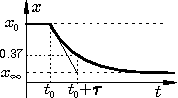
\includegraphics{./img/char/char_Schaltung1Grad.pdf} } \\
	\boxed{ \text{Lösung:}\quad x(t) = x_\infty + (x_0 - x_\infty) \exp\left(- \frac{t-t_0}{\tau}\right) }\\
	Mit Parameter aus ESB: C: $x_\infty = U_0(t)$, L: $x_\infty = I_0(t)$
	\\
	Beispiele: \hspace{3cm} $u_C(t) = A \cdot \sin(\omega t)$\\
	\pbox{5.0cm}{ 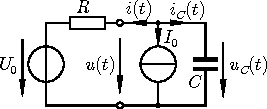
\includegraphics[scale = 0.8]{./img/Schaltung1Grad.pdf} \\ \\ $\dot u(t) = - \frac{u(t)}{RC} + \frac{U_0 + RI_0}{RC}$ }
	\pbox{3.0cm}{ 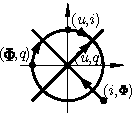
\includegraphics{./img/char/capsin.pdf} }\\



	\subsubsection{Dynamischer Pfad}
	\begin{tabular}{l|l}
		kapazitiv & induktiv \\ \hline
		$u_C$ stetig, $i_C$ springt & $i_L$ stetig, $u_L$ springt \\
		$\dot u(t) = - \frac{1}{C} \cdot i(t)$ & $\dot i(t) = - \frac{1}{L} \cdot u(t)$ \\ \midrule
		$i > 0 \Ra \dot u < 0 \Ra u$ fällt & $u > 0 \Ra \dot i < 0 \Ra i$ fällt \\
		$i < 0 \Ra \dot u > 0 \Ra u$ steigt & $u < 0 \Ra \dot i > 0 \Ra i$ steigt \\
		$i = 0 \Ra \dot u = 0 \Ra$ GGP & $u = 0 \Ra \dot i = 0 \Ra$ GGP\\
	\end{tabular}\\
	\\[0.5em]
	\pbox{6.0cm}{
	Zeitdauer auf linearen Pfaden:\\	
		\boxed{\Delta t = t_1 - t_0 = \tau \ln \left( \frac{x(t_0) - x_\infty}{x(t_1) - x_\infty} \right)} 
	} \quad
	\pbox{3.0cm} {
		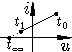
\includegraphics{./img/pfaddauer.pdf} }\\
	$x(t_0)$: Startwert,\quad $x(t_1)$: Zielwert,\quad $x_\infty$: (gedachter) GGP
	
	
	\subsection{Multivibrator mit $R_L = R_0 = R_1$}
	Relaxationsoszillator (NIK Polung beachten!):\\
	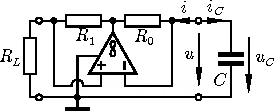
\includegraphics[scale = 0.8]{./img/astablemultivib.pdf} \ 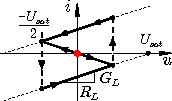
\includegraphics[scale = 0.9]{./img/char/char_astablemultivib.pdf}\\
	Flip-Flop (Bistabile Schaltung):\\
	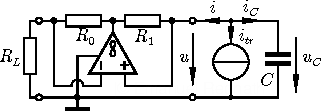
\includegraphics[scale = 0.8]{./img/bistablemultivib.pdf}  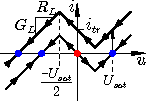
\includegraphics[scale = 0.9]{./img/char/char_bistablemultivib.pdf}

	
	\subsection{NIK allgemein (Polung beachten)}
	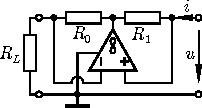
\includegraphics[scale = 0.85]{./img/NIK.pdf} \qquad 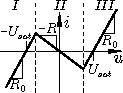
\includegraphics{./img/char/char_NIK.pdf}\\
	\begin{tabular}{cll}
	I & negative Sättigung $u_d < 0 \Leftrightarrow u_{out}=-U_{sat}$\\
	& $u = R_0 i - U_{sat}$\\ % < \frac{R_L}{R_L + R_1} \cdot U_{sat}$\\
	II & linearer Bereich $u_d = 0$\\
	& $u = - \frac{R_0}{R_1} R_L \cdot i$ \qquad \quad $-U_{sat} < \frac{R_L + R_1}{R_L}u < U_{sat}$\\
	III & positive Sättigung $u_d > 0 \Leftrightarrow u_{out}=U_{sat}$\\
	& $u = R_0 i + U_{sat}$ % < \frac{R_L}{R_L + R_1} \cdot U_{sat}$\\
	\end{tabular}

	\subsection{Eigenwerte(EW) $\lambda$ bestimmen}
	$\ma A \vec q = \lambda \vec q \ \Rightarrow \ (\ma A - \lambda \ma 1) \vec q = 0$ \quad mit Eigenwert $\lambda$ und Eigenvektor $\vec q$\\
	$\det (\ma{A}-\lambda \ma{1}) = 0$\\
	\\
	Vereinfachung für $2 \times 2$ Matrizen:\\
	\boxed{
	 \lambda_{1/2} = \frac{\mathrm{sp} \ma A}{2} \pm \sqrt{ \left( \frac{\mathrm{sp} \ma A}{2} \right)^2 - \det \ma A } } \quad \boxed{ \begin{array}{ll} \text{Wähle} \\ \bigl| \lambda_1 \bigr| < \bigl|\lambda_2 \bigr|  \end{array}}\\[0.5em]
	$\mathrm{Sp } \ma A = T = a_{11} + a_{22}$, \quad $\det \ma A = \Delta = a_{11} a_{22} - a_{12} a_{21}$\\
	\\
	Zeitkonstante $\tau = RC = GL$ % = -\frac{1}{\lambda}$


	\subsection{Eigenvektoren(EV) $\vec q$ bestimmen}
	$(\ma A-\lambda \ma 1) \vec q = 0 \ \Rightarrow \ \ma Q = \ker(\ma A-\lambda \ma 1)$ \\
	\fbox{ Merke: Eigenvektoren sind beliebig skalierbar! }
	\\
	Vereinfachung für $2 \times 2$ Matrizen, falls $\lambda_1 \ne \lambda_2$:\\
	\\
	\begin{tabular}{l|l}
	$a_{12} \ne 0:$ & $a_{21} \ne 0:$ \\ \midrule
	$q_{1/2} = \mvect{-a_{12} \\ a_{11} - \lambda_{1/2} }$ & $q_{1/2} = \mvect{a_{22} - \lambda_{1/2} \\ -a_{21} }$  \\
	\end{tabular}\\
	\\
	Falls $a_{12} = a_{21} = 0:$ $q_1 = \mvect{1 \\ 0} \quad q_2 = \mvect{0 \\ 1}$
	\fbox{ Eigenschaften EV (falls gefragt kann man das prüfen):  $\vec q_1 \perp \vec q_2 $}
	
	\subsection{Gleichgewichtspunkte(GGP) $\vec x_\infty$ bestimmen}
	$\vec x_\infty$: $\bs{ \dot {\vec x}} = 0 = \ma A \vec x_\infty + \ma B \vec v \quad \Ra \quad$ \boxed { \vec x_\infty = - \ma A^{-1} \ma B \vec v }\\[0.5em]
	Oder aus Schaltbild berechnen:\\
	Ersetze $C \ra LL$ und $L \ra KS$, berechne $\vec x = \vec x_\infty$
	

	\subsection{autonome(inhomogene) Systeme mit $\vec v = const.$}
	1. Fall $\ma A$ ist invertierbar ($\lambda_{1/2} \ne 0$)
	\begin{enumerate}\itemsep0pt
		\item Transformation auf homogenes System:\\
		\begin{tabular}{ll}
			$\vec x' = \vec x - \vec x_\infty$ & (gültig, da $\vec{\dot x}' = \vec{\dot x}$)\\
			$\vec x_\infty = - \ma A^{-1} \ma B \vec v$ & (oder aus Schaltbild berechnen)\\
			$\vec x'_0 = \vec x_0 - \vec x_\infty$ & Anfangswerte auch transformieren!\\
		\end{tabular}
		\item Löse homogenes System $\vec{\dot x}' = \ma A \vec x'$ 
		\item Gesamtlösung durch Rücktransformation: $\vec x = \vec x' + \vec x_\infty$\\
			$\Ra$ Verschiebung des Ursprungs um $\vec x_\infty$\\
	\end{enumerate}
	2. Fall $\ma A$ ist singulär ($\exists \lambda = 0$)
	\begin{enumerate}\itemsep0pt
		\item Transformation auf Normalform: $\vec{ \dot x} = \vec x \ma A + \ma B \vec v \quad \big|\  \ma Q^{-1} \cdot$ \\
		$\Ra \quad \vec{ \dot \xi} = \ma \Lambda \vec \xi + \vec v'$ \quad mit $\ma \Lambda = \mat{0 & 0 \\ 0 & \lambda}$\\
		\item Berechne Xi Lösungen: \\
		$\xi_2 = -\frac{v'_2}{\lambda} + \left(\xi_{0,2} + -\frac{v'_2}{\lambda} \right)\exp(\lambda t)$\\[0.5em]
		\begin{tabular}{l|l}
				Falls $v'_{01} = 0$ & Falls $v'_{01} \ne 0$ \\ \midrule
				$\xi_1 = const.$ & $\xi_1 = v'_1 \cdot t = \xi_{0,1}$\\
				$\xi_\infty = \vect{ iwas \\ -\frac{v'_2}{\lambda}}$ & Kein GGP! \\
		\end{tabular}
		\item Gesamtlösung durch Rücktransformation: $\vec x = \ma Q \cdot \xi$\\
	\end{enumerate}	



	\subsection{Nichtlineare dynamische Schaltungen 2. Grades}
	\begin{enumerate}\itemsep0pt
		\item DGL aufstellen: $\vec{\dot x} = \vec f(\vec x)$
		\item GGPs bestimmen: $\dot{\vec x} = \vec f(\vec x) \stackrel{!}= \vec 0$ \\
		\begin{tabular}{llll}
			$C:$ & $\dot u_C = 0$ & $\Rightarrow \ i_C = 0$ & $\Rightarrow$ LL\\
			$L:$ & $\dot i_L = 0$ & $\Rightarrow \ u_L = 0$ & $\Rightarrow$ KS\\
		\end{tabular}
		\item Linearisiere in $\vec x_\infty$:\\
		$\vec f(\vec x) \approx \vec f(\vec x_\infty) + \ma J (\vec x_\infty) \cdot (\vec x - \vec x_\infty)$
		\item Berechne EW und EV von $\ma J (\vec x_\infty)$ für jeden GGP
		\item Satz von Hartman:\\
				Falls von $\ma J(\vec x_\infty)$ der Realteil aller Eigenwerte ungleich null ist ($Re(\lambda) \ne 0$), dann verhält sich ein konservatives System in der Umgebung von $\vec x_\infty$ qualitativ genauso wie ein lineares System mit $\ma J(\vec x_\infty)$ als Systemmatrix.

	\end{enumerate}	
	



	\subsection{Normalform}
	Um DGL's 2ten Grades zu entkoppeln und auf zwei DGL's ersten Grades zurückzuführen.
	Transformiertes System = Diagonalisiertes System = Xi-System in Xi-Koordinaten.\\
	\boxed{ \underset{ \ma Q^{-1} \vec{\dot x}(t) }{\vec{ \dot \xi}(t)} = \underset{\ma Q^{-1} \ma A \ma Q}{\ma \Lambda} \cdot \underset{ \ma Q^{-1} \vec x(t) }{\vec \xi(t)} + \underset{ \ma Q^{-1} \ma B \vec v(t) }{\vec v'(t)} }\\
	$\ma Q$: Matrix der Eigenvektoren \quad $\ma \Lambda$: Diagonalmatrix der Eigenwerte.\\
	\begin{tabular}{l|l}
		Transformation: & Rücktransformation \\
		$\vec \xi(t) = \ma Q^{-1} \vec x(t)$ & $\vec x(t) = \ma Q \vec \xi(t)$\\
		$\ma \Lambda = \ma Q^{-1} \ma A \ma Q$ & $\ma A = \ma Q \ma \Lambda \ma Q^{-1}$\\
		$\vec v' = \ma Q^{-1} \ma B \vec v(t)$ & $\ma B \vec v = \ma Q \vec v'$\\
	\end{tabular}\\
	

\section{Komplexe Wechselstromrechnung }
Vorraussetzung: lineares, eingeschwungenes System mit sinusförmiger Erregung: $x(t) = \hat x \cdot \cos(\omega t + \varphi) = \hat x \cdot \sin(\omega t + \varphi + \frac{\pi}{2})$\\
Eigenschaften: eindeutig, linear, differenierbar ($\frac{\mathrm d}{\mathrm dt} = j \omega$)\\
Beispiel: $u_L = L \cdot \frac{\mathrm d}{\mathrm dt} i_l \ \Rightarrow \vec U_L = L \cdot j \omega \vec I_L$\\[0.5em]
\parbox{5.1cm}{\Large $e^{j\omega t} = \cos(\omega t) + j \sin(\omega t)$ \\[0.2em] $\omega = 2 \pi f$ \qquad $A = X_m=|X|$ \\[0.2em] \normalsize Komplexe Zahlen: $\frac{z_2}{a+jb} = \frac{z_2(a-jb)}{a^2+b^2}$ \quad $ \frac{1}{j}=-j $ }
\parbox{1.7cm}{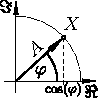
\includegraphics{./img/Zeiger.pdf}} \\
\framebox{
\begin{tabular}{ll}
	Zeiger: &\!\!\!\!\!\!$X = A \cdot \exp(j \varphi) = A \cdot \cos(\varphi) + A \cdot j \sin(\varphi)$\\[0.5em]
	Zeitsignal: &\!\!\!\!\!\!$x(t) = \Re[X \cdot \exp(j \omega t)] = A \cdot \cos(\omega t + \varphi)$\\
\end{tabular} }
\\[0.5em]
$\begin{array}{c|c|c|c|c|c|c|c|c}
x & 0 & \pi / 6 & \pi / 4 & \pi / 3 & \pi / 2 & \pi & \frac{3}{2}\pi & 2 \pi \\ \hline
\sin & 0 & \frac{1}{2} & \frac{1}{\sqrt{2}} & \frac{\sqrt 3}{2} & 1 & 0 & -1 & 0 \\
\cos & 1 & \frac{\sqrt 3}{2} & \frac{1}{\sqrt 2} & \frac{1}{2} & 0 & -1 & 0 & 1 \\   
\tan & 0 & \frac{\sqrt{3}}{3}&	1				 &	\sqrt{3} & \infty & 0 & - \infty & 0\\  
\end{array}$\\
\\
$\underset{\text{Impedanz}}{Z(j\omega)} = \underset{\text{Resistanz}}{R(j\omega)} + \underset{\text{Reaktanz}}{jX(j\omega)}$: Impedanz $U = Z \cdot I $\\
$\underset{\text{Admittanz}}{Y(j\omega)} = \underset{\text{Konduktanz}}{G(j\omega)} + \underset{\text{Suszeptanz}}{jB(j\omega)}$: Admittanz $I = Y \cdot U$\\


\everymath{\displaystyle}
\begin{tabular}{l|ll}
	& $Z$ & $Y$\\ \midrule
Widerstand & $R$ & $G = \frac{1}{R}$ \\
Kondensator & $\frac{1}{j \omega C}$ & $j \omega C$\\
Spule & $j \omega L$ & $\frac{1}{j \omega L}$ \\
Memristor & $M$ & $\frac{1}{M}$\\
\end{tabular}
\everymath{\textstyle}



Rechenregeln:
$A = a + j b = \hat A_m \exp(j \varphi)$\\
Radius $\hat A_m = \sqrt{a^2 + b^2}$\\

Mehrere Erregungen mit unterschiedlicher Kreisfrequenz:\\
Getrennte Zeigerrechnung für einzelne Frequenzen, dann zurücktransformieren und addieren.

\subsection{Oszillatoren}
autonome Schaltung 2. Grades mit nur einem instabile GGP.\\
\begin{tabular}{l|lll}
Van der Pol($L||C$) & Stückweise & fast harmon. & Relax.\\
$\ma J(\vec x_\infty)=$ & $\ma J(\vec x_\infty)=$ & $\lambda_{1/2} =$ & $L\ra 0$\\
$\mat{\frac{1}{RC} & -\frac{1}{C} \\ \frac{1}{L} & 0}$ & $\mat{0 & -\frac{1}{C} \\ \frac{1}{L} & \pm \frac{R}{L} }$ & $\pm \frac{R}{2L} \pm j \omega_0$\\
\end{tabular}




\subsection{Übertragungsfunktion $H(j\omega) = a + j b$}
$H(j \omega) = \frac{U_{out}}{U_{in}} = |H(j \omega)| \cdot \exp\bigl(j\varphi(\omega)\bigr)$\\

Bei Knotenspannungsanalyse:\\
$H(j\omega) = \frac{U_{out}}{U_{in}} = \frac{U_{Km}}{I_n}\cdot G = \frac{(-1)^{n+m} \det \ma Y_{nm}(j\omega)}{\det \ma Y_k(j\omega)}\cdot G$\\[0.5em]
Wichtige Regeln:\\
$20\log_{10} \left( \frac{1}{a} \right) = -20\log_{10} \left( a \right)$ \qquad $\log_{10}(1) = 0$\\ $20\log_{10} \left( \sqrt{a} \right) = 10\log_{10} a$ \\[0.5em]
Faktorisieren: $H(j \omega) = \prod H_i(j \omega)$ damit gilt:\\
$v(\omega) = \sum v_i(\omega)$ \qquad $\varphi(\omega) = \sum \varphi_i(\omega)$\\

$\sphericalangle H(j \omega) = \varphi(\omega) = \begin{cases}
\arctan \frac{b}{a} & \text{für } a > 0 \\
+ \frac{\pi}{2} & \text{für } a= 0, b > 0 \\
- \frac{\pi}{2} & \text{für } a = 0, b < 0 \\
\arctan \frac{b}{a} + \pi & \text{für } a < 0, b \ge 0 \\
\arctan \frac{b}{a} - \pi & \text{für } a < 0 , b < 0
\end{cases}$\\
$\arctan \left( - \frac{b}{a} \right) = - \arctan \left( \frac{b}{a} \right)$
\\[6em]
$H(p) = k \cdot \frac{p}{p^2 + p \frac{\omega_0}{Q} + \omega^2_0 }$:\\ 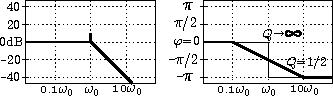
\includegraphics{./img/bodesquare.pdf}




\subsection{Pol-Nullstellen-Diagramm (PN-Diagramm)}
Polstellen $\times$, Nullstellen $\circ$\\
Polstellen = Eigenfrequenzen = Eigenwerte.\\
Polstellen haben negativen Realteil $\Ra$ Schaltung Stabil.


\subsection{Ortskurven}
Berechne Markante Punkte von $Y(j\omega)$ oder $Z(j\omega)=\frac{U}{I}=H(j\omega)$\\
\begin{tabular}{lll}
$\Re Z(j0)$ & $\Im Z(j0)$\\
$\Re Z(j\infty)$ & $\Im Z(j\infty)$\\
$\Re Z(j\omega_0)$ & $\Im Z(j\omega_0)$\\
\end{tabular}


	\subsection{Leistung und Energie}
	Differenzielle Energie: $\diff E = p(t) \diff t = u(t) \cdot i(t) \diff t$\\
	Wirkleistung: $P_w = \frac{1}{T} \int\limits_0^T p(t) \diff t$\\
	Für lineare resistive Schaltungen: $P_w = R \cdot I^2_{eff} = \frac{U^2_{eff}}{R}$\\
	Komplexe Leistung: $P = \frac12 UI^* = P_w + j P_B$\\

% Ende der Spalten
\end{multicols}



\hrule \hrule

\begin{multicols}{3}
\section{Lösen von homogenen DGLs}
Gegeben: Homogene Differnetialgleichungen der Form $\vec{\dot x} =  \ma A \vec x$ \\
mit Anfangswerten $x_{0,1}$ und $x_{0,2}$\\[2em]
\boxed{ \boldsymbol{\lambda_1 \ne \lambda_2 \in \R} } \qquad  \boxed{ \bigl| \lambda_1 \bigr| < \bigl|\lambda_2 \bigr|  \quad \Ra \vec q_2 \text{,,schneller''} } \\[1.5em]
$\vec x(t) = x_{0,1} \cdot \exp(\lambda_1 t) \cdot \vec q_1 + x_{0,2} \cdot \exp(\lambda_2 t) \cdot \vec q_2$\\[1.5em]
\begin{tabular}{l|l|l|l|l}
	Matrix $\Lambda$ & Eigenwerte & $\vec x = 0$ & Name & Portrait\\ \midrule \midrule
	{$\mat{\lambda_1 & 0 \\ 0 & \lambda_2}$} & $\lambda_1 < 0 < \lambda_2$ & instabil & Sattelpunkt & \pbox{3.0cm}{ 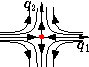
\includegraphics{./img/char/PP_Sadle.pdf} }\\ \midrule
		& $\lambda_2 < 0, \lambda_1 < 0 $ & stabil & Knoten 2 & \pbox{3.0cm}{ 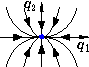
\includegraphics{./img/char/PP_stableNode.pdf} }\\ \midrule
		& $0 < \lambda_1, 0 < \lambda_2 $ & instabil & Knoten 2 & \pbox{3.0cm}{ 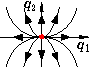
\includegraphics{./img/char/PP_unstableNode.pdf} }\\ \midrule
	\multirow{2}{*}{$\mat{0 & 0 \\ 0 & \lambda_2}$} & $\lambda_1 = 0,\ \lambda_2 < 0$ & stabil & Kamm & \pbox{3.0cm}{ 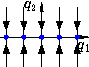
\includegraphics{./img/char/PP_stableLine.pdf} }\\ \midrule
	 & $\lambda_1 = 0,\ \lambda_2 > 0$ & instabil & Kamm & \pbox{3.0cm}{ 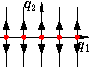
\includegraphics{./img/char/PP_unstableLine.pdf} }\\
\end{tabular}
\vspace{2em}\\

%\vspace{5em}\\

\boxed{ \boldsymbol{\lambda_1 = \lambda_2 \in \R} }\\
$\ma Q' = \mat{ \vec q'_1 & \vec q'_2} = \mat{ -a_{12} & -a_{12} \\ \frac{a_{11} - a_{22}}{2} & \frac{a_{11} - a_{22}}{2} -1 } = \mat{ \vect{\text{Eigen-} \\ \text{vektor}} & \vect{\text{Haupt-} \\ \text{vektor}}}$\\
$\vec x(t) = \left[ \ma 1 + (\ma A - \lambda \ma 1) \cdot t \right] \cdot \exp(\lambda t) \cdot \mvect{x_{0,1} \\ x_{0,2}}$\\[0.5em]
\begin{tabular}{l|l|l|l|l}
	Matrix $\Lambda$ & Eigenwerte & $\vec x = 0$ & Name & Portrait\\ \midrule \midrule
	\multirow{2}{*}{$\mat{\lambda & 0 \\ 0 & \lambda}$} & $\lambda < 0$ & stabil & Knoten 1 & \pbox{3.0cm}{ 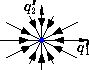
\includegraphics{./img/char/PP_stableStarNode.pdf} }\\ \midrule
	& $\lambda > 0$ & instabil & Knoten 1 & \pbox{3.0cm}{ 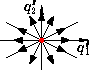
\includegraphics{./img/char/PP_unstableStarNode.pdf} }\\ \midrule
	\multirow{2}{*}{$\mat{\lambda & 1 \\ 0 & \lambda}$} & $\lambda < 0$ & stabil & Knoten 3 & \pbox{3.0cm}{ 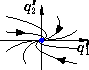
\includegraphics{./img/char/PP_stableWhirlNode.pdf} }\\ \midrule
	& $\lambda > 0$ & instabil & Knoten 3 & \pbox{3.0cm}{ 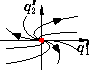
\includegraphics{./img/char/PP_unstableWhirlNode.pdf} }\\ \midrule
	$\mat{0 & 0 \\ 0 & 0}$ & $\lambda = 0$ & stabil & Ruheebene & \pbox{3.0cm}{ 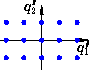
\includegraphics{./img/char/PP_stableZero.pdf} }\\ \midrule
	$\mat{0 & 1 \\ 0 & 0}$ & $\lambda = 0$ & instabil & Ruhegerade & \pbox{3.0cm}{ 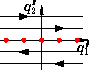
\includegraphics{./img/char/PP_unstableZero.pdf} }\\
\end{tabular}


\boxed{ \boldsymbol{\lambda_1 = \lambda^*_2 = \alpha + \beta j \in \C} } \qquad \boxed{ \ma Q' = \mat{\Re \vec q_1 & \Im \vec q_1} = \mat{ \vec q_r & \vec q_j} }\\

$\begin{array}{rl} \vec x(t) & = x_{0,1} \cdot e^{\alpha t} \cdot \left[ \cos (\beta t) \vec q_r - \sin(\beta t) \cdot \vec q_j \right] + \\ & +\, x_{0,2} \cdot e^{\alpha t} \cdot \left[ \sin (\beta t) \vec q_r + \cos(\beta t) \cdot \vec q_j \right] \end{array}$\\
\begin{tabular}{l|l|l|l|l}
	Matrix $\Lambda$ & Eigenwerte & $\vec x = 0$ & Name & Portrait\\ \midrule \midrule
	\multirow{2}{*}{$\mat{\alpha & -\beta \\ \beta & \alpha}$} & $\alpha < 0,\ \beta \ne 0$ & stabil & Strudel & \pbox{3.0cm}{ 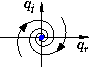
\includegraphics{./img/char/PP_stableFocus.pdf} }\\ \midrule
	& $\alpha > 0,\ \beta \ne 0$ & instabil & Strudel & \pbox{3.0cm}{ 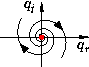
\includegraphics{./img/char/PP_unstableFocus.pdf} }\\ \midrule
	$\mat{0 & -\beta \\ \beta & 0}$ & $\alpha = 0,\ \beta \ne 0$ & stabil & Wirbel & \pbox{3.0cm}{ 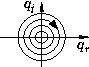
\includegraphics{./img/char/PP_Whirl.pdf} }\\ 
\end{tabular}
\vspace{1em}\\
Zeitverlauf immer von $\vec q_j$ nach $\vec q_r$ bzw. von $\vec q_r$ nach $-\vec q_j$\\[4em]
Lösung für \emph{inhomogene DGL}($\vec v \ne 0$) mit singulärer Matrix $\ma A$ (nicht entkoppelbar):\\
\begin{tabular}{l|l|l|l|l}
$\mat{0 & 0 \\ 0 & \lambda_2}$ & $\lambda_1 = 0,\ \lambda_2 < 0$ & instabil & Kamm & \pbox{3.0cm}{ 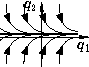
\includegraphics{./img/char/PP_unstableLine2.pdf} }\\
$\mat{0 & 1 \\ 0 & 0}$ & $\lambda = 0$ & instabil & Knoten & \pbox{3.0cm}{ 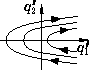
\includegraphics{./img/char/PP_unstableZero2.pdf} }\\
\end{tabular}



% Ende der Spalten
\end{multicols}

\hrule \hrule

\begin{multicols}{3}
\section{Anhang}

	\subsection{Mathematik}
		Matritzen:\\
		$\ma{A} = \frac{1}{\det \ma{A} } \begin{bmatrix}
		a_{22} & -a_{12}\\ 
		-a_{21} & a_{11}
		\end{bmatrix}$
		\\ \\
		%\subsection{Quadratische Lösungsformel}
		Quadratische Lösungsformel: \\
		$ax^2+ bx + c = 0$ :\\
		\boxed{x_{1/2} = \frac{-b \pm \sqrt{b^2 - 4ac}}{2a} } \\ \\
		Einfache quadratische Lösungsformel: \\
		$x^2 + px + q = 0$ :\\
		\boxed{x_{1/2} = -\frac{p}{2} \pm \sqrt{\left (  \frac{p}{2}\right )^2 - q}} \\

	\subsection{Ohmsches Gesetz}
	\begin{tabular}{ll}
		Basis:  & \\
		$U = R \cdot I$  &  $I = G \cdot U$ \\
		& \\
		Spannungsteiler:  &  Stromteiler: \\
		$u_2 = \frac{R_2}{R_1+R_2} \cdot  u_1$  &   $\frac{i_1}{i_ges} = \frac{R-ges}{ R_1} = \frac{G_1}{u}$ \\
	\end{tabular}
	
	\subsection{Zweitorbeschreibungen}
	\begin{tabular}{cll}
	I & Widerstandsbeschreibung:\\
	& $\left.\begin{matrix} u_1\\ u_2\end{matrix}\right]=\left.\begin{matrix} r_1(i_1,i_2)\\ r_2(i_1,i_2) \end{matrix}\right] = \ma{R} \cdot \left.\begin{matrix} i_1\\ i_2 \end{matrix}\right]$\\
	II & Leitwertsbeschreibung:\\
	& $\left.\begin{matrix} i_1\\ i_2\end{matrix}\right]=\ma{G} \cdot \left.\begin{matrix} u_1\\ u_2 \end{matrix}\right]$\\
	III & Hybridebeschreibung:\\
	& $\left.\begin{matrix} u_1\\ i_2\end{matrix}\right]=\ma{H} \cdot \left.\begin{matrix} i_1\\ u_2 \end{matrix}\right]$\\
	IV & Inverse Hybridbeschreibung:\\
	& $\left.\begin{matrix} i_1\\ u_2\end{matrix}\right]=\ma{H'} \cdot \left.\begin{matrix} u_1\\ i_2 \end{matrix}\right]$\\
	V & Kettenbeschreibung:\\
	& $\left.\begin{matrix} u_1\\ i_1\end{matrix}\right]=\ma{A} \cdot \left.\begin{matrix} u_2\\ -i_2 \end{matrix}\right]$\\
	VI & Inverse Kettenbeschreibung:\\
	& $\left.\begin{matrix} u_2\\ i_2\end{matrix}\right]=\ma{A'} \cdot \left.\begin{matrix} u_1\\ -i_1 \end{matrix}\right]$\\
	\end{tabular}

% Ende der Spalten
\end{multicols}

% Dokumentende
% ======================================================================
\end{document}




Halde:

\begin{tabular}{l|l|l|l|l}
	Matrix $\Lambda$ & Eigenwerte & $\vec x = 0$ & Name & Portrait\\ \midrule
	\multirow{3}{*}{$\mat{\lambda_1 & 0 \\ 0 & \lambda_2}$} & $\lambda_1 < 0 < \lambda_2$ & instabil & Sattelpunkt & \pbox{3.0cm}{ 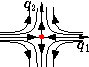
\includegraphics{./img/char/PP_Sadle.pdf} }\\
		& $\lambda_2 < \lambda_1 < 0 $ & stabil & Knoten 2 & \pbox{3.0cm}{ 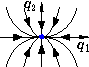
\includegraphics{./img/char/PP_stableNode.pdf} }\\
		& $0 < \lambda_1 < \lambda_2 $ & instabil & Knoten 2 & \pbox{3.0cm}{ 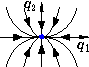
\includegraphics{./img/char/PP_stableNode.pdf} }\\
	\multirow{2}{*}{$\mat{0 & 0 \\ 0 & \lambda_2}$} & $\lambda_1 = 0,\ \lambda_2 < 0$ & stabil & Kamm & \pbox{3.0cm}{ 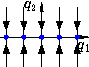
\includegraphics{./img/char/PP_stableLine.pdf} }\\	
	 & $\lambda_1 = 0,\ \lambda_2 > 0$ & instabil & Kamm & \pbox{3.0cm}{ 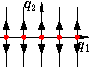
\includegraphics{./img/char/PP_unstableLine.pdf} }\\	\midrule
	\multirow{2}{*}{$\mat{\lambda & 0 \\ 0 & \lambda}$} & $\lambda < 0$ & stabil & Knoten 1 & \pbox{3.0cm}{ 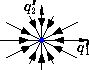
\includegraphics{./img/char/PP_stableStarNode.pdf} }\\
	& $\lambda > 0$ & instabil & Knoten 1 & \pbox{3.0cm}{ 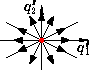
\includegraphics{./img/char/PP_unstableStarNode.pdf} }\\
	\multirow{2}{*}{$\mat{\lambda & 1 \\ 0 & \lambda}$} & $\lambda < 0$ & stabil & Knoten 3 & \pbox{3.0cm}{ 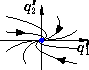
\includegraphics{./img/char/PP_stableWhirlNode.pdf} }\\
	& $\lambda > 0$ & instabil & Knoten 3 & \pbox{3.0cm}{ 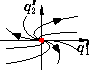
\includegraphics{./img/char/PP_unstableWhirlNode.pdf} }\\
	$\mat{0 & 0 \\ 0 & 0}$ & $\lambda = 0$ & stabil & Ruheebene & \pbox{3.0cm}{ 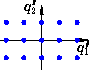
\includegraphics{./img/char/PP_stableZero.pdf} }\\
	$\mat{0 & 1 \\ 0 & 0}$ & $\lambda = 0$ & instabil & Ruhegerade & \pbox{3.0cm}{ 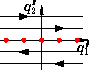
\includegraphics{./img/char/PP_unstableZero.pdf} }\\ \midrule
	\multirow{2}{*}{$\mat{\alpha & -\beta \\ \beta & \alpha}$} & $\alpha < 0,\ \beta \ne 0$ & stabil & Strudel & \pbox{3.0cm}{ 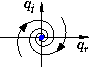
\includegraphics{./img/char/PP_stableFocus.pdf} }\\
	& $\alpha > 0,\ \beta \ne 0$ & instabil & Strudel & \pbox{3.0cm}{ 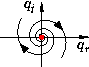
\includegraphics{./img/char/PP_unstableFocus.pdf} }\\
	$\mat{0 & -\beta \\ \beta & 0}$ & $\alpha = 0,\ \beta \ne 0$ & stabil & Wirbel & \pbox{3.0cm}{ 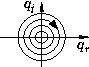
\includegraphics{./img/char/PP_Whirl.pdf} }\\
\end{tabular}




	\subsection{Lösung für hom. DGL }
	Für Gleichungen der Form $\vec{\dot x} =  \ma A \vec x$ mit Anfangswerten $x_{0,1},x_{0,2}$\\[0.5em]
	$\lambda_1 \ne \lambda_2$: $\vec x(t) = x_{0,1} \cdot \exp(\lambda_1 t) \cdot \vec q_1 + x_{0,2} \cdot \exp(\lambda_2 t) \cdot \vec q_2$\\[0.5em]
	$\lambda_1 = \lambda_2$: $\vec x(t) = \left[ \ma 1 + (\ma A - \lambda \ma 1) \cdot t \right] \cdot \exp(\lambda t) \cdot \mvect{x_{0,1} \\ x_{0,2}}$\\[0.5em]
	$\lambda_1 = \lambda^*_2$:
	 $\begin{array}{rl} \vec x(t) & = x_{0,1} \cdot e^{\alpha t} \cdot \left[ \cos (\beta t) \vec q_r - \sin(\beta t) \cdot \vec q_j \right] + \\ & +\, x_{0,2} \cdot e^{\alpha t} \cdot \left[ \sin (\beta t) \vec q_r + \cos(\beta t) \cdot \vec q_j \right] \end{array}$\\







